\chapter{Related research}
\label{chap:related}
With the increase of smartphone usage it is no surprise that a lot of research has been done considering beamforming algorithms. Many different algorithms have been proposed to use to perform beamforming with \cite{vanveen1988, griffiths1982, krim1996}. In this chapter, related research relevant to this topic will be discussed.

First common methods and the state of the art in beamforming research for acoustic and speech enhancement will be discussed. Then the different measures to evaluate the performance of these algorithms are introduced and to conclude ways to implement localization on the smartphones and distributed computation of the beamforming algorithm will be looked into.

\section{Beamforming Algorithms}
\label{sec:rel_beamformers}

Microphone arrays are a common way to improve sound quality; the diversity in the received signals is exploited by setting different gains to each microphone, depending on the location of the source and on the auxiliary sources and noise. This is generally referred to as beamforming. There are different beamforming algorithms each with their own advantages and disadvantages. The delay-and-sum beamformer (DSB) is one of the earliest beamforming algorithms. It is a "fixed" beamformer, meaning that it only adapts to the locations of the microphones and the desired source. It delays and optionally weighs the microphone signals based on the distances and the speed of sound and the attenuation of the soundwave respectively before taking the average of the signals. The MVDR beamformer is one of the most widely used beamformers and can be used for both speech dereverberation and noise reduction \cite{naylor2010speech}.

\subsection{Delay-and-sum Beamformer}
The delay-and-sum beamformer (DSB) is an important approach to dereverberation and provides a reference to compare other methods with. The expected improvement in the Direct to Reverberant Ratio (DRR) of the DSB only depends on the distance between the source and  the array and the seperation of the microphones and does not depend on reverberation time, which is the time it takes for the reverberant energy to drop to 60 dB below the original level. When the microphones are seperated by a half wavelength, perfect dereverberation is achieved \cite{naylor2010speech}. For spatially white noise only, the DSB is the optimal beamformer \cite{brandstein2001}.

White noise in general is a random signal with a constant power spectral density. It has a constant bandwidth and does not depend on the frequency \cite{carter2013}. Spatially white noise means that the noise is uncorrelated amongst all sensors in the array \cite{krim1996}.

\subsection{Minimum variance distortionless response Beamformer}
The minimum variance distortionless response (MVDR) beamformer \cite{naylor2010speech} is one of the most widely used beamformers. This beamforming algorithm can suppress coherent noise sources well. However, in a spatially white noise field, the MVDR beamformer reduces to a DSB  \cite{naylor2010speech}. The MVDR is also excessively sensitive to source location and microphone gains \citep{ba2007}.

There are multiple proposed variations on the standard MVDR beamformer. The first variation on the steered beamformer based locators with an increased accuracy in reverberate rooms is proposed by Ba et al. \cite{ba2007}. This algorithm is specifically designed for directional microphones in a teleconference setting. The algorithm uses voice activity detection to differentiate between speech and noise in the sound at the input of the beamformer. The noise component of the input will be used to update the covariant matrix of the beamformer. The block diagram of this algorithm can be found in figure \ref{fig:emvdr}. 

In the research by Ba et al. \cite{ba2007} a comparison is made between an MVDR beamformer with and without gain compensation for the microphone directivity. However, only circular microphone arrays are considered in this paper. The proposed eMVDR, which stands for enhanced MVDR, algorithm with the directivities included, outperforms the traditional MVDR in all ten of the experimented scenarios.
\begin{figure}
	\centering  
	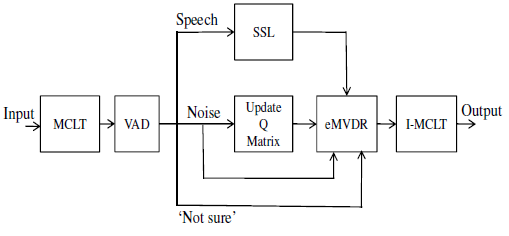
\includegraphics[scale=1]{Blockdiagram_emvdr.png}
	\caption{Block diagram of the eMVDR \cite{ba2007}} 
	\label{fig:emvdr}
\end{figure}
A different variation on the MVDR, which includes directivities in the beamformer, is proposed by Gaubitch et al. \cite{gaubitch2014}. This research also concludes that including the directivities in the beamformer significantly increases the performance of the beamformer. 



\subsection{Other beamforming algorithms}
Another beamforming algorithm, which is proposed by Martinez et al. \cite{martinez2015}, uses an eigenfilter structure to focus on regions instead of just an angle. The consequence of this variation is an increase in the robustness of the beamformer.

Another kind of beamformer is the generalized sidelobe canceller (GSC) \cite{griffiths1982}. One of the disadvantages of this beamformer is the robustness problem \cite{brandstein2001}. The beamformer suffers from target-signal cancellations due to errors in the steering vector. The generalized sidelobe canceller computes the weight factors in a different way than the MVDR beamformer resulting in a much lower complexity.

\section{Evaluation of the Beamforming techniques}
To investigate the performance of our algorithms, the results will be evaluated using different intelligibility measures \cite{taal2010,rix2001}.
The measures used to evaluate a beamformer are power related measures and intelligibility measures. The power related measure show a ratio between powers, for example the SNR shows the ratio of signal to noise. This can be used to determine if a beamforming algorithm suppresses the noise while keeping the signal power the same. Intelligibility measures determine the extend to which a signal is understandable for speech applications. In this thesis the beamforming algorithms are used to enhance speech, which is why the intelligibility measures are interesting to investigate.

Different power related measures exist which can be used to investigate the performance of a beamformer. A few of them are:

\begin{itemize}
\item Global SNR[dB]
\item Segmental SNR [dB]
\item White noise gain
\item Array-gain
\end{itemize}

The global and segmental SNR are calculated by determining the ratio between the power of the signal and the power of the noise. The global SNR uses the complete signal to determine this ratio. The segmental SNR calculates the average SNR of only those frames of the sound signal which exhibit an SNR larger than $0 dB$ \cite{brandstein2001}. The segmental SNR measures the amplitude distortion of the sound signal and will therefore be well correlated with perceived distortions. 

The shows the ability of a beamformer to suppress spatially uncorrelated noise \cite{brandstein2001}. White noise gain is defined as the output power due to unit variance white noise in the sensor \cite{vanveen1988}.  The white noise gain is represented by $\textbf{w}^H\textbf{w}$. If the white noise gain is high, the beamformer output will have a poor SNR due to white noise contributions. 

The array-gain shows the improvement of the signal-to-noise ratio between one of the microphones and enhanced output of the array and can be calculated as follows:

\begin{equation}
G_{A} = \frac{\text{SNR}_\text{{array}}}{\text{SNR}_\text{microphone}}
\end{equation}

\nomenclature{$G_\text{A}$}{Array-gain}
\nomenclature{$SNR$}{Signal-to-noise ratio [dB]}

An intelligibility measure that shows a good correlation with speech intelligibility is the Short-Time Objective Intelligibility measure (STOI) \cite{taal2010, taal2011}. STOI is based on the correlation between short-time segments of the clean and processed signal. The short-time segments used were approximately $400 ms$. This algorithms was specifically designed for a sample-rate of $10000 Hz$ to cover the relevant frequency range for speech. The STOI is expressed in the range $0$ to $1$ where a higher value means that the signal is more intelligible.

\nomenclature{STOI}{Short-Time Objective Intelligibility measure}

Another widely used intelligibility measure is Perceptual Evaluation of Speech Quality (PESQ). PESQ predicts the perceived quality that would be given to the processed signal by subjective listening tests. This measure shows a high correlation with the subjective Mean Opinion Scores (MOS) \cite{rix2001, itu2010}.

The mean opinion score is a test that results in an indication of the quality of a phone call on a scale from $1$ to $5$, where $1$ stands for bad and $5$ stands for excellent. There are guidelines, given by ITU-T recommendation $P.800$ \cite{ituquality1998}, for the environment of the speaker that should be followed when conducting such a test.

It is expected that an improvement in SNR results in an improvement in MOS \cite{itumos1996}. This means that the PESQ should also improve since MOS and PESQ show a high correlation. 

\nomenclature{MOS}{Mean opinion scores}
\nomenclature{PESQ}{Perceptual evaluation of speech}